\documentclass[a4paper,10pt]{article}
\usepackage[utf8]{inputenc}
\usepackage{graphicx}
\usepackage[section]{placeins}
\usepackage{tabularx}
\usepackage[vmargin=3cm, hmargin=2cm]{geometry}
\usepackage[T1]{fontenc} 
\usepackage[ngerman]{babel}

\title{Pflichtenheft}
\author{Simon Bischof \and Jan Haag \and Adrian Herrmann \and Lin Jin \and Tobias Schlumberger \and Matthias Schnetz}

\begin{document}

\maketitle
\newpage
\tableofcontents
\newpage

\section{Produktübersicht}

Das Produkt ist ein Werkzeug zur Analyse und Korrektheitsprüfung von Programmen. Der Benutzer hat die Möglichkeit, in eine grafische Oberfläche ein Programm mit der im Anhang spezifizierten While-Sprache zu laden und mit Annotationen zu versehen, die als Vor- und Nachbedingungen geprüft werden.

\section{Zielbestimmung}
\subsection{Interpreter / Run-time Checker}
\subsubsection{Musskriterien}
\begin{itemize}
  \item schrittweise Ausführung eines Programms
  \item Inspektion des aktuellen Programmzustands durch den Benutzer
  \item Prüfung von Zusicherungen in Programmen zur Laufzeit
\end{itemize}
\subsubsection{Sollkriterien}
\begin{itemize}
  \item Auswertung von Formeln mit Quantoren über eingeschränkten Bereich
\end{itemize}
\subsubsection{Kannkriterien}
\begin{itemize}
  \item Auswertung von benutzerdefinierten Ausdrücken über Programmzustand
  \item Auswertung von Formeln mit Quantoren mit Hilfe eines Beweisers
\end{itemize}

\subsection{Grafische Benutzeroberfläche}
\subsubsection{Musskriterien}
\begin{itemize}
  \item englische Sprache
  \item Steuerung der einzelnen Komponenten des Systems
  \item Anzeige von fehlgeschlagenen Laufzeitprüfungen
\end{itemize}
\subsubsection{Kannkriterien}
\begin{itemize}
  \item Syntax Highlighting
\end{itemize}
\subsubsection{Abgrenzungskriterien}
\begin{itemize}
  \item nur Optionen in der grafischen Oberfläche, die einen echten Mehrwert bieten
\end{itemize}

\subsection{Verifikation}
\subsubsection{Musskriterien}
\begin{itemize}
  \item formale Verifikation eines Programms mit Hilfe eines Beweisers
\end{itemize}

\subsection{While-Sprache}
\subsubsection{Musskriterien}
\begin{itemize}
  \item Zuweisungen, Bedingten Anweisungen und Schleifen
  \item Nur die Typen Ganzzahl, Boolean und Arrays
  \item Keinen Heap
  \item Keine Nebenläufigkeit
\end{itemize}
\subsubsection{Kannkriterien}
\begin{itemize}
  \item Programmiersprache unterstützt Methodenaufrufe
\end{itemize}

\subsection{Annotationssprache}
\subsubsection{Musskriterien}
\begin{itemize}
  \item Ausdrücke in Annotationen ähnlich wie in der Programmiersprache, zusätzlich Quantoren
  \item Zusicherungen erlauben Aussagen der Prädikatenlogik
  \item Annotationen assert und assume
\end{itemize}
\subsubsection{Sollkriterien}
\begin{itemize}
  \item syntactic sugar für Vor- und Nachbedingungen, (In)Varianten und globale Annahmen
\end{itemize}


\section{Produkteinsatz}
Das Produkt ermöglicht dem Benutzer die Analyse eines Programmes, das in der im Anhang beschriebenen While-Sprache geschrieben ist. Dabei ist es sowohl möglich, die Anweisungen des Programms schrittweise oder komplett zu durchlaufen und dabei zur Laufzeit auf im Programmcode durch Annotationen eingebettete Zusicherungen zu überprüfen, als auch die formale Verifikation des Programms mithilfe des automatischen Theorembeweisers Z3 von Microsoft. 

\subsection{Anwendungsbereiche}
\begin{itemize}
  \item Formale Verifikation von Programmen
  \item Testen von Programmen der While-Sprache
\end{itemize}

\subsection{Zielgruppen}
\begin{itemize}
  \item Informatiker
\end{itemize}

\section{Produktumgebung}
\subsection{Software}
\begin{itemize}
  \item Java Runtime Environment SE 6 oder höher
  \item Windows NT 4.0 oder neuer oder Betriebssystem mit Wine
\end{itemize}

\subsection{Hardware}
\begin{itemize}
  \item mindestens 512 MB Arbeitsspeicher
\end{itemize}

\subsection{Schnittstellen}
\begin{itemize}
  \item Das Produkt erzeugt Dateien im SMT-LIB 2.0 Format als Schnittstelle zu Z3
\end{itemize}

\section{Funktionale Anforderungen}
\subsection{Übersicht}
\begin{tabular}{| l | l |}
\hline
/F10/ & Anzeige von Quelltext\\
/F20/ & Syntax Highlighting\\
/F30/ & Veränderung des Quelltextes\\
/F40/ & Speichern des Quelltextes in eine Datei\\
/F50/ & Laden eines Programms aus einer Datei\\
/F60/ & Erkennen und Anzeigen von Syntaxfehlern\\
/F70/ & Erkennen und Anzeigen von Typfehlern\\
/F80/ & Ausführen eines Programms\\
/F90/ & Setzen und Entfernen von Breakpoints\\
/F100/ & Programmabbruch bei Fehler mit Anzeige des Fehlers\\
/F110/ & Anzeige des Programmzustands\\
/F120/ & Auswertung von benutzerdefinierten Ausdrücken\\
/F130/ & Auswertung der Annotationssprache\\
/F140/ & Anzeige der Beweisereinstellungen\\
/F150/ & Laden der Beweisereinstellungen aus einer Datei\\
/F160/ & Speichern der Beweisereinstellungen in eine Datei\\
/F170/ & Beweiser starten und Ergebnis anzeigen\\
\hline
\end{tabular}
\subsection{Details}
\begin{description}
\item[/F10/] Anzeige von Quelltext\\
Der Benutzer sieht den Quelltext des aktuellen Programms in der grafischen Oberfläche.
\item[/F20/] Syntax Highlighting\\
Teile des angezeigten Quelltextes werden abhängig von ihrer Bedeutung in unterschiedlichen Farben angezeigt.
\item[/F30/] Veränderung des Quelltextes\\
Der Benutzer kann den angezeigten Quelltext verändern oder einen neuen Quelltext eingeben.
\item[/F40/] Speichern des Quelltextes in eine Datei\\
Der Benutzer kann den eingegebenen Quelltext ($\to$/F30/) in eine Datei speichern. Dabei gibt der Benutzer den gewünschten Speicherort und den Dateinamen über eine grafische Oberfläche an.
\item[/F50/] Laden eines Programms aus einer Datei\\
Der Benutzer kann ein Quellcode eines Programms aus einer Datei laden. Hierbei gibt der Benutzer die zu ladende Datei über eine grafische Oberfläche an.
\item[/F60/] Erkennen und Anzeigen von Syntaxfehlern\\
Falls der aktuell angezeigte Quelltext Syntaxfehler enthält, wird dies dem Benutzer angezeigt, wenn er die Programmausführung oder die Beweisführung anfordert.
\item[/F70/] Erkennen und Anzeigen von Typfehlern\\
Falls der aktuell angezeigte Quelltext Typfehler enthält, wird dies dem Benutzer angezeigt, wenn er die Programmausführung oder die Beweisführung anfordert.
\item[/F80/] Ausführen eines Programms\\
Die Anweisungen im aktuell angezeigten Quelltext können ausgeführt werden. Dabei sind folgende Ausführungsmodi möglich:\\
\begin{tabularx}{\textwidth}{lX}
\leftskip=4cm
Single Step & Es wird auf eine Interaktion des Benutzers nur eine Anweisung ausgeführt.\\
Run until Breakpoint & Es werden sequentiell alle Anweisungen ausgeführt, bis das Programm beendet ist oder ein Breakpoint ($\to$/F90/) erreicht wird.\\
\end{tabularx}
\item[/F90/] Setzen und Entfernen von Breakpoints\\
Der Benutzer kann Breakpoints zur Pausierung eines Programmdurchlaufs an Stellen des angezeigten Quellcodes setzen und wieder entfernen.
\item[/F100/] Programmabbruch bei Fehler mit Anzeige des Fehlers\\
Tritt ein Fehler zur Laufzeit des Programms auf, wird die Ausführung abgebrochen und der Fehler dem Benutzer angezeigt.
\item[/F110/] Anzeige des Programmzustands\\
Der Benutzer sieht während der Ausführung eines Programms den aktuellen Inhalt aller globalen und lokalen Variablen. Die Anzeige wird nur aktualisiert, wenn das Programm die Ausführung pausiert.
\item[/F120/] Auswertung von benutzerdefinierten Ausdrücken\\
Der Benutzer kann Ausdrücke über den aktuellen Programmzustand auswerten lassen.
\item[/F130/] Auswertung der Annotationssprache\\
Während der Programmausführung werden die Bedingungen der Annotationssprache ausgewertet. Schlägt eine Überprüfung fehl, so wird die Ausführung des Programms angehalten und dem Benutzer angezeigt, welche Bedingung falsch ist.
\item[/F140/] Anzeige der Beweisereinstellungen\\
Der Benutzer kann die aktuellen Einstellungen ($\to$/P10/) für die Ausführung des Beweisers ($\to$/F170/) anzeigen lassen. Diese werden vor der Anzeige aus einer Datei geladen ($\to$/F150/) und bei einer Veränderung wieder in eine Datei geschrieben ($\to$/F160/).
\item[/F150/] Laden der Beweisereinstellungen aus einer Datei\\
Die Einstellungen für die Ausführung des Beweisers ($\to$/P10/) werden automatisch aus einer Datei gelesen.
\item[/F160/] Speichern der Beweisereinstellungen in eine Datei\\
Die Einstellungen ($\to$/P10/) werden in eine Datei gespeichert.
\item[/F170/] Beweiser starten und Ergebnis anzeigen\\
Der Benutzer kann den Beweiser für das aktuelle Programm starten. Das Ergebnis des Beweisers wird dem Benutzer nach Beendigung des Beweisvorgangs angezeigt.
\end{description}

\section{Produktdaten}
Es sind folgende Daten des Benutzers zu Speichern:
\begin{description}
\item[/D10/] Benutzereinstellungen
\begin{itemize}
  \item Timeout in Sekunden für den Beweiser
  \item Speicherbegrenzung in Megabyte für den Beweiser
\end{itemize}
\end{description}

\section{Produktleistungen}
\begin{itemize}
  \item Verifikation- und Falsifikationsrückmeldungen vom Beweiser müssen korrekt sein, in anderen Fällen soll dem Benutzer mitgeteilt werden, dass der Beweiser das Problem nicht lösen kann
\end{itemize}

\section{Weitere nichtfunktionale Anforderungen}
Die Lizenz von Z3 erlaubt ausschließlich eine nicht-kommerzielle Benutzung.

\section{Qualitätsanforderungen}
\begin{itemize}
  \item Programmiersprache muss erweiterbar sein
  \item mögliche Anbindung anderer Beweiser, die das SMT-LIB 2.0 Format unterstützen
  \item unter (durch benutzerdefinierte Einstellungen vorgegebene, $\to$/F140/) Normalbedingungen stürzt das Programm nicht ab
  \item jede Aktion gibt in jedem Fall eine Rückmeldung an den Benutzer
\end{itemize}

\section{Globale Testfälle und Testszenarien}
Folgende Funktionssequenzen sind zu überprüfen:
\begin{description}
\item[/T10/] Eingabe des leeren Programms $\to$ keine Syntaxfehler
\item[/T20/] Eingabe des leeren Programms, Beweisvorgang starten $\to$ Verifikation durch den Beweiser
\item[/T30/] Eingabe des leeren Programms, Annotation \texttt{\_(ensure false)}, Programmausführung $\to$ Annotationsbedingung schlägt fehl
\item[/T40/] Eingabe des leeren Programms, Annotation \texttt{\_(ensure true)}, Programmausführung $\to$ Annotationsbedingung schlägt nicht fehl
\item[/T50/] Eingabe eines beliebigen Programms, Annotation \texttt{\_require false}, Programmausführung $\to$ Annotationsbedingung schlägt fehl, Programmausführung wird abgebrochen
\item[/T60/] Eingabe eines Programms mit Zuweisung \texttt{x = 1}, Annotation \texttt{\_(require x>0)}, Programmausführung $\to$ Annotationsbedingung schlägt nicht fehl
\item[/T70/] Eingabe eines Programms mit Syntaxfehler $\to$ Anzeige des Syntaxfehlers
\item[/T80/] Eingabe eines Programms mit while-Schleife oder if-Konstrukt, deren Bedingung kein boolean ist $\to$ Anzeige des Typfehlers
\item[/T90/] Eingabe eines Programms mit einem Operator, der nur auf Ganzzahlen definiert ist und auf einen boolean angewendet wird $\to$ Anzeige des Typfehlers
\item[/T100/] Eingabe eines Programms mit einem Operator, der nur auf booleans definiert ist und auf Ganzzahlen angewendet wird $\to$ Anzeige des Typfehlers
\item[/T110/] Eingabe eines Programms mit einer Zuweisung eines boolean an eine Ganzzahl $\to$ Anzeige des Typfehlers
\item[/T120/] Eingabe eines Programms mit einer Zuweisung einer Ganzzahl an einen boolean $\to$ Anzeige des Typfehlers
\item[/T130/] Eingabe eines Programms mit einer Zuweisung einer Ganzzahl oder eines boolean an ein Array $\to$ Anzeige des Typfehlers
\item[/T140/] Eingabe eines Programms mit einem Vergleichsoperator, der auf zwei unterschiedliche Typen ausgeführt wird $\to$ Anzeige des Typfehlers
\item[/T150/] Eingabe eines Programms mit Zuweisung \texttt{y = 2x}, Annotation \texttt{\_ensure(y==2x)}, Beweisvorgang starten $\to$ Verifizierung durch den Beweiser
\item[/T160/] Eingabe eines Programms mit Zuweisung \texttt{y = 2x}, Annotation \texttt{\_ensure(y\%2==0)}, Beweisvorgang starten $\to$ Verifizierung durch den Beweiser
\item[/T170/] Eingabe eines längeren Programms ohne Schleifen und ohne if-Konstrukt, Eingabe von Annotationen, die in jedem Fall wahr sind, Beweisvorgang starten $\to$ Verifizierung durch den Beweiser
\item[/T180/] Eingabe eines längeren Programms ohne Schleifen und mit if-Konstrukt, Eingabe von Annotationen, die in jedem Fall wahr sind, Beweisvorgang starten $\to$ Verifizierung durch den Beweiser
\item[/T190/] Eingabe eines längeren Programms mit Schleifen, Eingabe von Annotationen, die in jedem Fall wahr sind, Beweisvorgang starten $\to$ Verifizierung durch den Beweiser
\item[/T200/] Eingabe eines Programms mit Annotation \texttt{\_(ensure x!=x)}, Beweisvorgang starten $\to$ Falsifikation durch den Beweiser
\item[/T210/] Eingabe eines längeren Programms mit Schleife (z.B. russische Multiplikation, Maximum der Zahlen in einem Array), Eingabe von Annotationen, die in mindestens einem Fall falsch sind, Beweisvorgang starten $\to$ Falsifikation durch den Beweiser
\item[/T220/] Eingabe eines Programms mit Annotation \texttt{\_(require x\%2==0)}, Zuweisung \texttt{y = 2*(x/2)} und Annotation \texttt{\_ensure(x==y)}, Beweisvorgang starten $\to$ Verifikation durch den Beweiser
\item[/T230/] Eingabe eines Programms ohne Annotation, Beweisvorgang starten $\to$ Beweisvorgang wird nicht gestartet
\item[/T240/] Eingabe eines Programms mit Division durch 0, Ausführung des Programms $\to$ Anzeige des Laufzeitfehlers
\item[/T250/] Eingabe eines Programms mit Deklaration und Initialisierung eines Arrays, fehlerhafter Arrayzugriff, Ausführung des Programms$\to$ Anzeige des Laufzeitfehlers
\end{description}

\section{Systemmodelle}
\subsection{Übersicht}
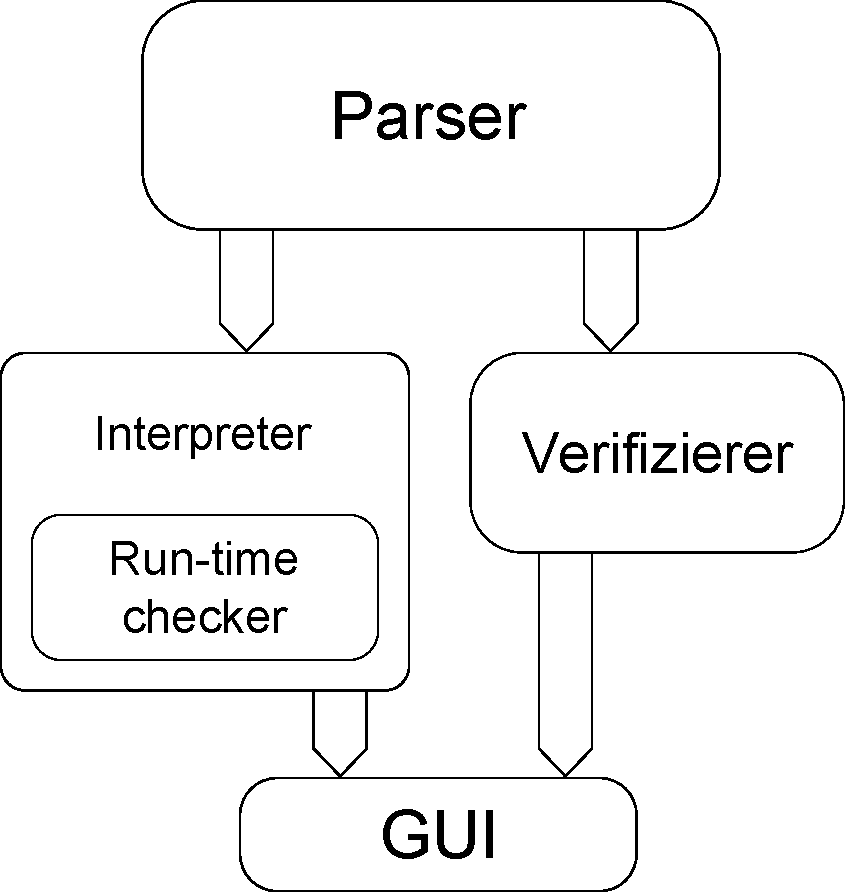
\includegraphics{systemmodelle.pdf}

\section{Benutzungsoberfläche}
\begin{figure}
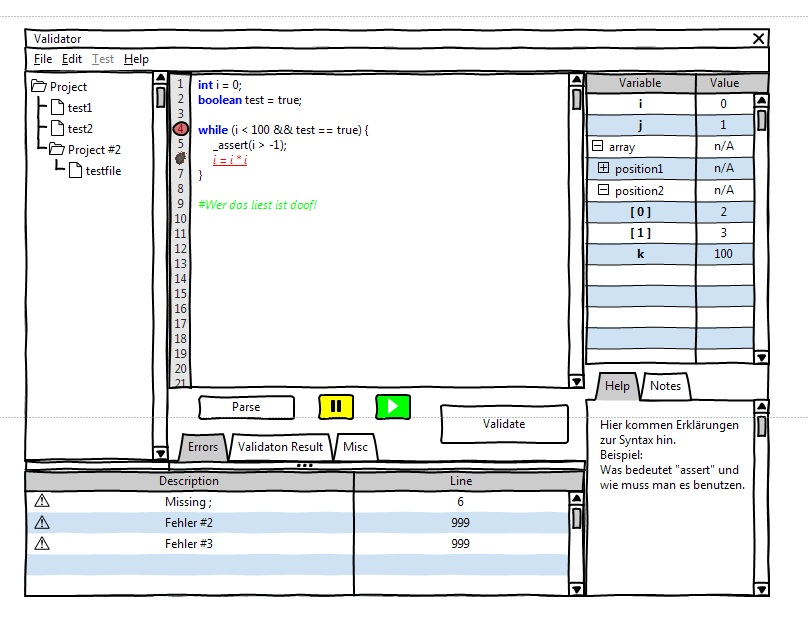
\includegraphics[width=\textwidth]{images/mockup1.jpg}
\end{figure}
\begin{figure}
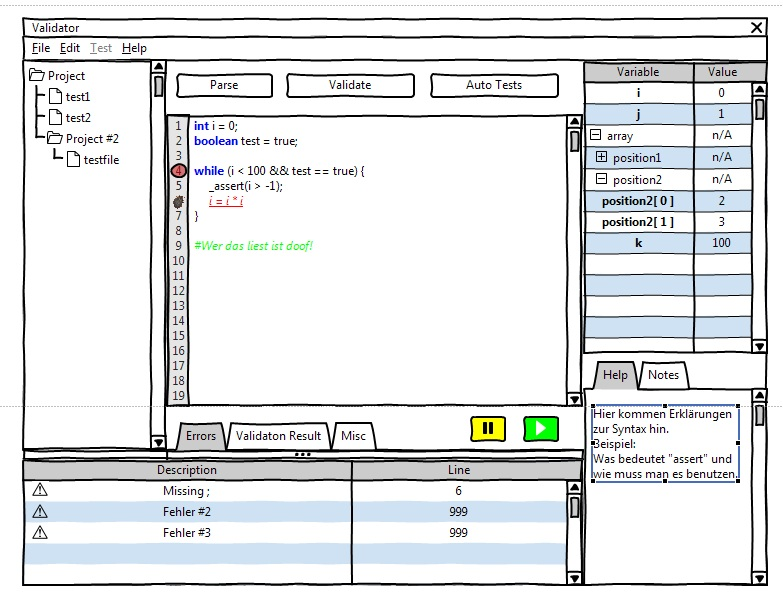
\includegraphics[width=\textwidth]{images/mockup2.jpg}
\end{figure}
\begin{figure}
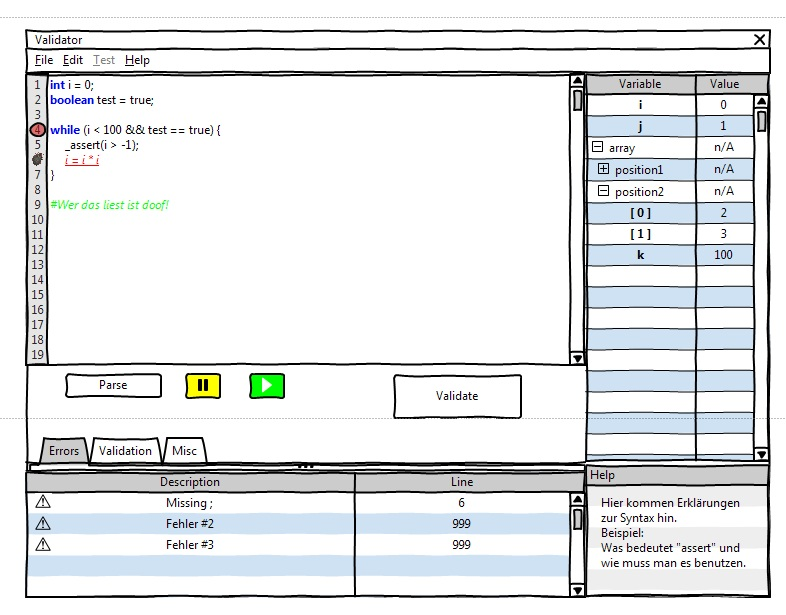
\includegraphics[width=\textwidth]{images/mockup3.jpg}
\end{figure}

\section{Spezielle Anforderungen an die Entwicklungsumgebung}
\begin{description}
  \item[Versionsverwaltung] Git
  \item[Kommunikation] E-Mail, Wiki
  \item[Dokumente] \LaTeX
  \item[Programmiersprache] Java
\end{description}

\section{Zeit- und Ressourcenplanung}
\subsection{Phasenverantwortliche}
\begin{tabular}[h]{| l | r |}
\hline
\textbf{Phase} & \textbf{Verantwortliche(r)}\\
\hline
Pflichtenheft & Tobias\\
\hline
Entwurf & Adrian\\
\hline
Implementierung & Simon, Jan\\
\hline
Validierung & Lin\\
\hline
Abschlusspräsentation & Matthias\\
\hline
\end{tabular}


\section{Ergänzungen}
\subsection{While-Sprache}
\subsubsection{Variablentypen}
\begin{description}
\item[Ganzzahl] ganze Zahl beliebiger Genauigkeit.
\item[Boolean] Wahrheitswert, entweder wahr oder falsch.
\item[Array] eine Zusammenfassung mehrerer Variablen eines Variablentyps. Die maximale Anzahl möglicher Variablen in einem Array ist nach erster Festlegung konstant.
\end{description}
\subsubsection{Sprachkonstrukte}
\begin{tabularx}{\textwidth}{| l | X |}
\hline
\textbf{Konstrukt} & \textbf{Bedeutung}\\
\hline
if-else & Ausführung bestimmter Anweisungen, falls eine Bedingung erfüllt ist. Ausführung anderer Anweisungen, falls die Bedingung nicht erfüllt ist.\\
\hline
while & Wiederholte Ausführung von bestimmten Anweisungen, wenn eine Bedingung erfüllt ist.\\
\hline
Methoden & Definition einer Folge von Anweisungen mit Parametern, die zu einem anderen Zeitpunkt im Programmablauf aufgerufen werden können, und einen Wert zurückgeben.\\
\hline
einzeilige Kommentare & Annotation, die keinen Einfluss auf die Quelltextverarbeitung haben.\\
\hline
\end{tabularx}
\subsubsection{Operatoren}
\begin{tabularx}{\textwidth}{| l | X | l | X |}
\hline
\textbf{Operator} & \textbf{Eingabetypen} & \textbf{Ergebnistyp} & \textbf{Funktion}\\
\hline
\texttt{==} & 2 Variablen desselben Typs & Boolean & Prüft \texttt{T1} und \texttt{T2} auf Gleichheit, falls sie vom selben Variablentyp sind. Arrays sind gleich, wenn alle Elemente der tiefsten Ebene des Arrays gleich sind.\\
\texttt{!=} & 2 Variablen desselben Typs & Boolean & Prüft \texttt{T1} und \texttt{T2} auf Ungleichheit, falls sie vom selben Variablentyp sind. Liefert denselben Wert wie die Negation von \texttt{==}.\\
\texttt{=} & 1 Variable und ein Ausdruck & ? & Weist der Variable den Wert des Ausdrucks zu, wenn dieser Wert vom selben Variablentyp ist, wie die Variable.\\
\hline
\texttt{<} & 2 Ganzzahlen, \texttt{Ganzzahl1} und \texttt{Ganzzahl2} & Boolean & Prüft, ob \texttt{Ganzzahl1} kleiner als \texttt{Ganzzahl2} ist.\\
\texttt{>} & 2 Ganzzahlen, \texttt{Ganzzahl1} und \texttt{Ganzzahl2} & Boolean & Prüft, ob \texttt{Ganzzahl1} größer als \texttt{Ganzzahl2} ist.\\
\texttt{<=} & 2 Ganzzahlen, \texttt{Ganzzahl1} und \texttt{Ganzzahl2} & Boolean & Prüft, ob \texttt{Ganzzahl1} kleiner oder gleich \texttt{Ganzzahl2} ist.\\
\texttt{>=} & 2 Ganzzahlen, \texttt{Ganzzahl1} und \texttt{Ganzzahl2} & Boolean & Prüft, ob \texttt{Ganzzahl1} größer oder gleich \texttt{Ganzzahl2} ist.\\
\texttt{+} & 1 Ganzzahl, \texttt{Ganzzahl} & Ganzzahl & Gibt \texttt{Ganzzahl} zurück.\\
\texttt{-} & 1 Ganzzahl, \texttt{Ganzzahl} & Ganzzahl & Gibt -\texttt{Ganzzahl} zurück.\\
\texttt{+} & 2 Ganzzahlen, \texttt{Ganzzahl1} und \texttt{Ganzzahl2} & Ganzzahl & Addiert \texttt{Ganzzahl1} und \texttt{Ganzzahl2}.\\
\texttt{-} & 2 Ganzzahlen, \texttt{Ganzzahl1} und \texttt{Ganzzahl2} & Ganzzahl & Subtrahiert \texttt{Ganzzahl2} von \texttt{Ganzzahl1}.\\
\texttt{*} & 2 Ganzzahlen, \texttt{Ganzzahl1} und \texttt{Ganzzahl2} & Ganzzahl & Multipliziert \texttt{Ganzzahl1} mit \texttt{Ganzzahl2}.\\
\texttt{/} & 2 Ganzzahlen, \texttt{Ganzzahl1} und \texttt{Ganzzahl2} & Ganzzahl & Dividiert \texttt{Ganzzahl1} durch \texttt{Ganzzahl2}. Das Ergebnis wird zur Null hin gerundet.\\
\texttt{\%} & 2 Ganzzahlen, \texttt{Ganzzahl1} und \texttt{Ganzzahl2} & Ganzzahl & Liefert den Rest der Ganzzahldivision von \texttt{Ganzzahl1} durch \texttt{Ganzzahl2}.\\
\hline
\texttt{!} & 1 Boolean, \texttt{Boolean} & Boolean & Negiert den Wert von \texttt{Boolean}.\\
\texttt{\&} & 2 Boolean, \texttt{Boolean1} und \texttt{Boolean2} & Boolean & Liefert die Konjunktion von \texttt{Boolean1} und \texttt{Boolean2}.\\
\texttt{|} & 2 Boolean, \texttt{Boolean1} und \texttt{Boolean2} & Boolean & Liefert die Disjunktion von \texttt{Boolean1} und \texttt{Boolean2}.\\
\hline
\end{tabularx}
\subsubsection{Sonstige Spracheigenschaften}
\begin{itemize}
  \item Lexical Scoping
  \item sequentelle Komposition
  \item Kurzauswertung von logischen Operatoren
\end{itemize}

\subsection{Annotationssprache}
Die Annotationssprache besteht aus Ausdrücken der While-Sprache mit Quantoren und zusätzlich den folgenden Konstrukten:\\
\begin{tabularx}{\textwidth}{| l | X |}
\hline
\texttt{require} & Stellt eine Vorbedingung vor Schleifen oder Methoden dar.\\
\texttt{ensure} & Stellt eine Nachbedingung nach Schleifen oder Methoden dar.\\
\texttt{assert} & Stellt eine Bedingung an der aktuellen Stelle im Programmablauf dar.\\
\texttt{assume} & Stellt eine globale, als wahr angenommene Aussage dar.\\
\hline
\end{tabularx}


\section{Glossar}
\begin{description}
\item[Anweisung (Programm)] Eine syntaktisch korrekte Vorschrift, die bei der Abarbeitung des Programms auszuführen ist.
\item[Beweiser] Ein Programm, das versucht die Gültigkeit eines Theorems zu überprüfen. Ein Beispiel für ein solches Programm ist $\to$Z3.
\item[Kurzauswertung] Die Auswertung eines Ausdrucks wird abgebrochen, sobald der Wert des Ausdrucks bekannt ist.
\item[Lexical Scoping] Auf eine lokale Variable kann nur in ihrem lexikalischen Sichtbarkeitsbereich Bezug genommen werden.
\item[sequentielle Komposition] Hintereinanderausführung von mehreren Anweisungen.
\item[SMT-LIB 2.0] Ein Standardformat zur Beschreibung von Satisfiability Modulo Theories Problemen, d.h. Formeln der Prädikatenlogik erster Stufe.
\item[Z3] Ein $\to$Beweiser von Microsoft.
\end{description}

\end{document}
